\chapter{Reconstructing Cancer Progression Models}
In Figure \ref{fig:CRC}, there is an example of the evolution of Colon Rectal Cancer (CRC). 
The progression modes are multiple and the study of these is central in the discourse 
of so-called personalized medicine. Always talking about CRC The concept of staging 
must also be introduced. The progression of the tumor occurs in several steps, in 
detail of CRC are identified tendentially 4, each with its sub-stages, which lead from 
the initial state to the now uncontrolled development and metastasis of the tumor also 
in other organs.

\begin{figure}[!ht]
    \centering
    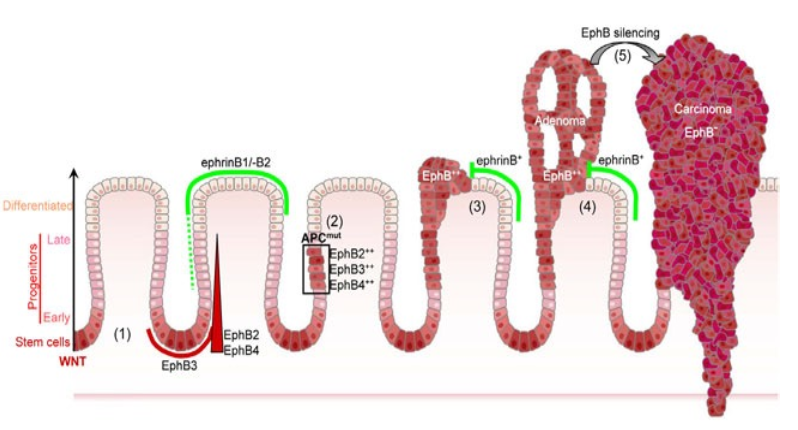
\includegraphics[width=0.5\linewidth]{img/CancerProgression/CRC.png}
    \caption{CRC Standard Progression}
    \label{fig:CRC}
\end{figure}

In this context, the study of images is also interesting, both through a committee of doctors 
who determine the extent of tumor progression, and, more computationally, using machine learning 
models and artificial intelligence techniques for image analysis. A good hypothesis, on most
types of cancer, is that the tumour progresses through \textbf{stages} by accumulating 
alterations affecting gene function and interactions. The following conclusions can be drawn:
\begin{itemize}
    \item The malfunction of individual genes cannot cause cancer. It has been understood that 
        a tumour is the result of multiple malfunctions of different genes;
    \item Cancer develops through multiple evolutionary pathways, so it is a problem to 
        where it actually develops;
    \item The alterations can be categorized in various ways, but among the main ones are:
        \begin{itemize}
            \item \textbf{Somatic mutations}: is a mutation at the DNA level of any cell in 
                the body. If the affected cell is still able to divide, the mutation is 
                transmitted to all cells resulting from it by mitosis. In this case the 
                organism will consist of a population of normal cells and one of mutated cells;
            \item \textbf{Copy number variation} (CNV): the phenomenon where sections of the
                genome are repeated and the number of replications in the genome varies from
                individual to individual. The variation of the number of copies is a type of
                structural variation: specifically, it is a type of duplication or deletion 
                event that affects a considerable number of base pairs, involving for example over-expression of certain proteins;
        \end{itemize}
        These, and many other events are due to countless factors, so the causes of cancer 
        progression can be really multiple
\end{itemize}

So, this whole modelling study is essential for drug development and for therapeutic decisions,
for example, for the same type of cancer, patients in different stages/stages of different 
progressions respond differently to different treatments.

Cancer cells are like other cells and can therefore be studied as individual replicators. 
The purpose is the same as normal cells, that is they have the objective to reproduce must
therefore:
\begin{enumerate}
    \item \textbf{Grow}: through energy consumption and nutrients;
    \item \textbf{Live long and prosper}, and therefore limit/avoid apoptosis;
    \item \textbf{Move}: in the case of cancer cells this is done by metastasis.
\end{enumerate}
A cancer cell is therefore essentially a cell which has exchanged a series of behaviors, 
dictated by its genetic make-up, for others more "successful" in its microenvironment,
unfortunately the concept of "successful" for the cell is a problem for the organism. 

By succeeding in replicating, these cells give rise to a new (\textbf{sub})\textbf{clonal}
population that continues to expand, thus generating neoplastic growth, or the abnormal 
growth of cells that leads to cancer.

Over the years, external causes of cancer have also been discovered. This adds further 
complexity to the studies.

It is now necessary to understand what are the \textbf{hallmarks} of cancer, the so-called 
cancer hallmarks. Cancer hallmarks represent a "new" mode of operation, giving cancer cells 
forms of selective advantage. These are described as follows:
\begin{itemize}
    \item \textbf{Self-sufficiency in growth signals}: remembering that at the cellular level
        signals are received by cells via proteins;
    \item \textbf{Insensitivity to anti-growth signals} that seek to limit uncontrolled tumor
        growth;
    \item \textbf{Avoid programmed cell death}: avoiding apoptosis reported by p53;
    \item \textbf{Unlimited replicative potential};
    \item \textbf{Making angiogenesis}: the process that leads to the formation of new blood
        vessels from other pre-existing vessels, sustained. This tells the circulatory system to 
        create blood vessels near the tumor so that it can better supply growth substances;
    \item \textbf{Tissue invasion} and \textbf{Metastasis};
    \item \textbf{Deregulate metabolism} (and that's what is being studied with FBA)
    \item \textbf{Evading the immune system}, which reacts not only with apoptosis but also 
        with many other operations;
    \item \textbf{Lead to genome instability}.
\end{itemize}
All these points are extreme behaviors that a normal cell would have anyway to grow, move 
and live long.

When it comes to cancer progression, we can draw a parallel with Darwin’s study of evolution. 
We can see how it starts with a certain normal cell that in a certain micro-environment at a
certain moment of time divides, accumulating in the various micro-environments various mutations 
and creating the tumor situation. A clone arrives and survives when it is "better" than the 
normal cells and other clones, eventually ending up with only clones.

The study of these problems is based on the data produced by sequencing and the creation of 
graphs such as that shown in Figure \ref{fig:CE}. 

\begin{figure}[!ht]
    \centering
    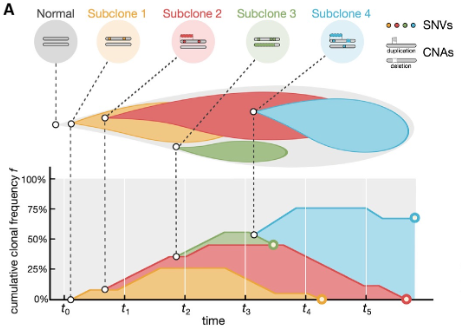
\includegraphics[width=0.5\linewidth]{img/CancerProgression/CE.png}
    \caption{Clonal Expansion}
    \label{fig:CE}
\end{figure}

Data is often problematic:
\begin{itemize}
    \item Missing data, for various technical reasons;
    \item Lack of useful time points. There are often very distant time points and with 
        uneven and increasing distances, mainly due to the method of experimentation used.
\end{itemize}

In general, these studies are useful to understand whether a particular cure is having the desired effect. For example, if we look at the Figure \ref{fig:Resistance}, we can see that 
some strains manage to survive the treatment. This can lead to a reappearance or the 
emergence of new mutations.

\begin{figure}[!ht]
    \centering
    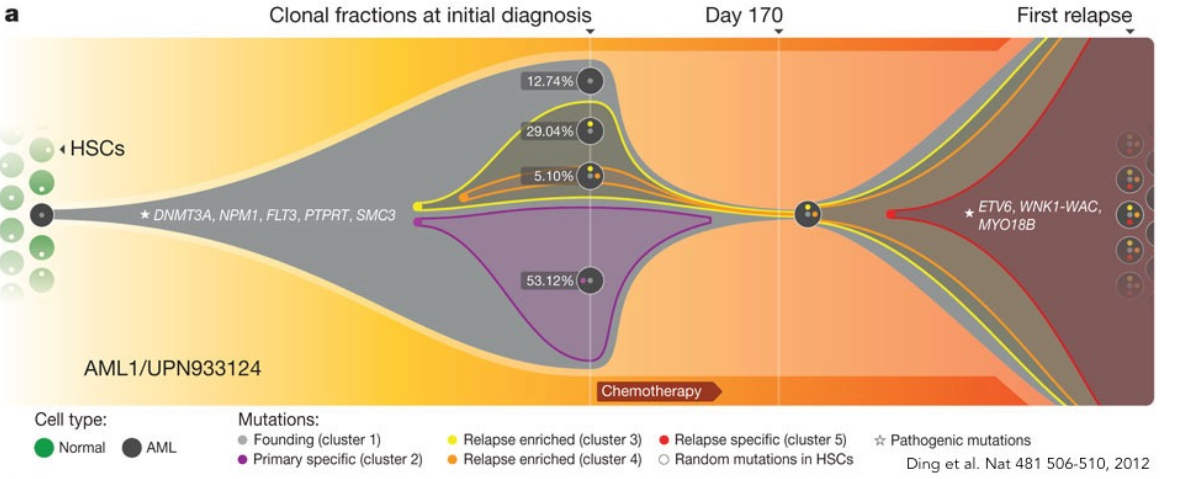
\includegraphics[width=0.5\linewidth]{img/CancerProgression/Resistance.png}
    \caption{Clonal Expansion and Resistance}
    \label{fig:Resistance}
\end{figure}

Another interesting aspect is the \textbf{Inter-Tumor} and \textbf{Intra-Tumor Heterogeneity} 
(ITH). The ITH is however a difficult subject to treat and study. Within a tumor in the same
patient there are variations, such as spatial and clonal heterogeneity, but there are also 
variations between the same tumor in different patients, thus having to make facets of 
heterogeneity.
\section{Cross Sectional Data}
A very important aspect in studying the evolution of cancer is to understand how data is collected 
and what it represents. In particular, there are two type of study:
\begin{enumerate}
    \item \textbf{ensemble-level}: Attempts to reconstruct a set of plausible precedence 
        relationships of events from patient data, which can be many. This is done from $n$ 
        independent cross-sectional data. We can imagine having a matrix with $n$ patient 
        genomes for the columns and $m$ "conductive events".
    \item \textbf{individual-level}: The attempt is to reconstruct a tumor cell population 
        from tissue samples using single-cell and phylogenetic techniques. In this case, we 
        start with $n$ samples of the same tumor, obtained from a biopsy, and sequenced by 
        bulk sequencing. The evolutionary tree is then obtained of a single tumor and study 
        the ancestral tumor and clones without generalizing selection, studying specifically 
        for the individual patient.
\end{enumerate}

We now want to go deeper into the ensemble-level, through cross-sectional data, as this type of 
data represents the majority of available cancer data. 

These data are collected through biopsies taken at the time of diagnosis. It is therefore a set 
of data that is collected only the first time and then you do not know what happens next. All 
these datasets are sorted so that results can be obtained on the tumour evolution. Inferring 
time information from such data is still an open challenge. 

We also know that these data are very noisy and often handled with machine learning techniques 
and neural networks. Another key aspect to consider is the missing data, which complicates matters 
further.

There are several databases that maintain and update information on cancer. The best known is 
\textbf{The Cancer Genome Atlas} (TCGA), which provides several portals to simplify access to data.
\subsection{Analysis}
We would like to answer the following questions:
\begin{enumerate}
    \item Can we reconstruct a progression model from cross-sectional data?
    \item What is actually contained in the datasets and what is actually contained in the 
        cross section, having changed a lot over the years?
    \item What kind of models can we rebuild?
\end{enumerate}

Let’s see how it is possible to reconstruct the progression models by using Direct 
Acyclic Graph (DAG), which encodes the accumulation of alterations and mutations. A useful 
library in this context is TRONCO, which contains various techniques and algorithms for the 
reconstruction of progression models.

In answering the first question, we can reconstruct a progression model from the creoss-sectional 
data. In addition, from these models, you can get tips on the correct therapies to use to treat 
a patient. The procedure for doing so is as follows:
\begin{itemize}
    \item • It starts from a \textit{Boolean matrix} where the columns are mutations and the rows 
        are tumors, indicating with 1 and 0 the presence or absence of a certain mutation in a certain tumor.
    \item A causal network is created where it is specified which mutation causes. Thus, a concept of
        "precedence" is obtained;
    \item The network then studies the mutual causality between mutations.
    \item The results are used to study pathway causality or phenotypes, or hallmarks, and therefore 
        have additional levels of abstraction from generic DAG.
\end{itemize}

As regards the second question, the public databases for cancer data must be used again. All these
databases address the problem of centralizing data and information, which until a few years ago 
were also quite expensive.

Obviously, in the field of cancer research, the most interesting information from databases, among 
the many available information, is that relating to mutations, which are usually inherited and 
persistent between successive generations of cancer cells. The most interesting mutations are usually 
those of somatic character, that is somatic mutations. In addition, it is more said that the probability
of occurrence of a given alteration is related to how functional it is to the development of the tumor,
having therefore that you have the mutations called driver and passenger, as well as different rates of 
tumor mutation. Of course, mutations can also be of various types:
\begin{itemize}
    \item The so-called single nucleotide variant (SNP), or single base mutations;
    \item Loss of heterozygosity, with loss of genomic regions, loss of smaller portions, 
        copy-number mutations etc$\dots$
    \item Whole deletions that are terminal or internal to the sequence
    \item Duplications of parts of sequences that can lead to tandem, where the duplications are next 
        to each other, or duplications where the duplicate portions are separated from each other by 
        another portion of the genome;
    \item Amplifications of genomic portions of intra-chromosomal and inter-chromosomal types; 
    \item Duplication of the entire genome.
\end{itemize}

To answer the third question we can use various studies which have defined the following models:
\begin{itemize}
    \item \textbf{Tree models}: these models are based on correlations;
    \item \textbf{Joint models}: mainly based on Bayesian models;
    \item \textbf{DAG models}: which are a generalization of the two previous models.
\end{itemize}

Let’s now look at some techniques developed in the DCB bicocca research laboratory:
\begin{itemize}
    \item \textbf{CAncer PRogression Extraction with Single Edges} (CAPRESE), for tree modelling.
    \item \textbf{CAncer PRogression Inference} (CAPRI), an extension of CAPRESE to work through 
        DAG models.
    \item These algorithms, plus other supporting features such as access to cBIO and TCGA, have 
        been collected in the R language library called \textbf{Translational ONCOlogy} (TRONCO).
\end{itemize}

Suppose you want to model a tumour progression in which two mutations occur, one called EGFR and 
then one called CDK. Two important assumptions must be made in order to proceed with the modelling:
\begin{enumerate}
    \item \textbf{Persistence assumption}: acquired mutations do not disappear. The EGFR mutation
        therefore gives a selective advantage, and then the clonal expansion is carried out. This 
        also increases the likelihood of acquiring a CDK mutation. When both mutations are present, 
        one species is selectively even more favoured;
    \item \textbf{Event selection assumption}: that is, events relevant for progression must be chosen 
        in advance. In practice, it is already known that a model with the EGFR and CDK mutations must 
        be studied. Limiting to a few combinations of events makes the reconstruction computationally 
        feasible, thus not using the entire multitude of data from oncology studies. It is then done a 
        sort of supervised study to find the driver mutations.
\end{enumerate}

Another key aspect in this study is that each patient has a different history of cancer evolution 
and progression. The actual input to the progression reconstruction algorithm can be thought of as 
a set of possible trajectories, that is, sequences of genomic alterations that accumulate in 
different ways. You must then proceed with counting and assigning the correct probabilities to each 
single occurrence of an event.

Over the years, various models have been developed to reconstruct tree or DAG models and all algorithms
need a measure to decide whether and how to include an arc in the reconstruction. In the above 
mentioned algorithms, it was chosen to use the theory of probabilistic causality.

Another key aspect in this study is that each patient has a different history of cancer evolution and
progression. The actual input to the progression reconstruction algorithm can be thought of as a set of 
possible trajectories, that is, sequences of genomic alterations that accumulate in different ways. You 
must then proceed with counting and assigning the correct probabilities to each single occurrence of an 
event.

Over the years, various models have been developed to reconstruct tree or DAG models and all algorithms 
need a measure to decide whether and how to include an arc in the reconstruction. In the above mentioned 
algorithms, it was chosen to use the theory of probabilistic causality.

The core of this theory is very simple. Two events $c$ and $e$, occurring respectively at time $t_c$ 
and $t_e$, are given with:
\begin{equation*}
    0 < P(c) \,\, \land \,\, P(e) < 1    
\end{equation*}
There is a \textit{prima facie} cause for $e$ if two properties are respected:
\begin{enumerate}
    \item The time priority property, that is:
        \begin{equation*}
            t_c < t_e
        \end{equation*}
        this ensures a time order between events.
    \item The property of probability growth, which tells us that the probability that the event $e$
        happens having happened to $c$ event is greater than that in which you do not have event $c$:
        \begin{equation*}
            P(e| \lnot c) < P(e|c)
        \end{equation*}
\end{enumerate}
These two properties, necessary but not sufficient, guarantee the directionality of the model.

In addition to the Suppes theory, both measurements and theoretical analyses are reinterpreted in
biologically plausible terms, possibly also by redefining selective advantage relationships. 

Let us then go into more detail on the basis for reconstructing the progression model. The already
anticipated prima facie cases can be of two types:
\begin{itemize}
    \item Authentic/genuine, the "correct ones";
    \item Spurious, "wrong" ones.
\end{itemize}
Therefore, the two conditions are only sufficient and not necessary. Also, speaking of cross-sectional
data, the time priority between events is not known, so the problem of reconstruction becomes more 
difficult. 

The problem becomes how to establish whether a given arc between two events corresponds or not to a 
false cause, and therefore should not be considered, since the interpretation of an arc will be that of 
a selective advantage relationship between genetic events.

In addition, a further complication is given by the fact that nothing ensures that we speak only of two
events but we can have complex combinations of causality between events. For this reason, in the CAPRI 
algorithm these situations are managed by means of boolean formulas, like the conjunctive formulas of 
the type used in the Bayesian conjunctive networks. 

The following are distinguished:
\begin{itemize}
    \item \textbf{Singleton}: where one mutation occurs before another and there is a causal relationship;
    \item \textbf{co-occurrence}: where more than one mutation occurs before another and there is a 
        causal relationship. Obviously, in this case the complexity increases.
\end{itemize}

In the CAPRI algorithm there is also a final condition, that is the condition for the selection
advantageous through patterns:
\begin{equation*}
    c e \Longleftrightarrow P(c) > P(e) \,\, \land P(e | c) < P(e| \lnot c)
\end{equation*}

We then start with a causal model with selective advantages, make observations on imperfect regularities
and frequency studies. More specifically, the inference of results is then obtained by statistical
techniques such as:
\begin{itemize}
    \item \textbf{boostrap}: a statistical technique of resampling with resampling to approximate the
        sample distribution of a statistic. It therefore allows you to approximate the mean and variance
        of an estimator, construct confidence intervals and calculate test p-values when the distribution
        of interest is not known;
    \item \textbf{p-value} and other tests.
\end{itemize}

Causal relationships between mutations are thus obtained, possibly also with the co-occurring effect 
of several mutations causing a third mutation.

For complex patterns it has been studied experimentally as the CAPRI algorithm which is able to understand
the causality between various mutations and represent them by Boolean formulas. The complexity of the 
model then leads back to the complexity of such formulas.

Boolean formulas are of the conjunctive normal form (CNF), or a conjunction of clauses, where clauses are
a disjunction of literal ones.

In order to limit complexity we must therefore highlight the most significant authentic relationships. 
The CAPRI algorithm is a combination of six steps which are responsible for producing a set of 
selectivity relationships and then cleaning up the generated model:
\begin{enumerate}
    \item Input data management;
    \item Pre-processing with addition of information, called lifting, to the raw model obtained from the
        data. We have a set $G$ of $n$ events from $m$ cross sectional samples, having therefore a Boolean 
        matrix $n \times m$. In this one we assume a set of hypotheses:
        \begin{equation*}
            \Phi = \{\phi_i \rhd e_i | 1 \leq i \leq k\}, \text{ con } k + n \ll m
        \end{equation*}
        Each individual $\phi \rhd e_i$ is used to increment the matrix into input by obtaining a 
        $D(\Phi)$ matrix that encodes optional selectivity relations as events.
    \item DAG node selection;
    \item DAG edge selection;
    \item There is then a phase of labeling the arcs. At this stage the coded selectivity relations are CNF 
        formulas, so they can be treated in a composite way by separately checking each conjunction. The algorithm
        includes in the construction arcs between two events $c$ and $e$ if and only if:
        \begin{equation*}
            P(c) - P(e) > 0 \,\,\land P(e | c) - P(e | \lnot c) > 0
        \end{equation*}
        and this is the main condition. Note that the probabilities are estimated from the data directly, through 
        a first step of boostrap. The reconstructed DAG contains all the correct selectivity relationships but also 
        several spurious ones, which are not yet eliminated.
        
        Each arc is labeled with a probability which is essentially the probability of observing a certain mutational 
        profile in a sample.
    \item Finally a likelihood fit phase. Recalling that the Suppes assumptions are only necessary to "filter" spurious
        relationships, ie false positives that have been included in the previous steps, we calculate a fit of maximum
        likelihood that includes a regularization term, The term may be chosen and calculated differently.

        Finally, a bootstrap pass is used to deduce the confidence intervals for each selectivity relation inferred.
\end{enumerate}

The CAPRI algorithm is correct and complete, since only true selectivity relationships deductible from the data are
reported.

It should always be remembered that the precedence relations which the algorithm deduces do not explain the 
mechanistic biochemical causes of a progression model, In fact, the algorithm only makes a statement that 
observing a given set of mutations increases the probability of seeing one later.